\documentclass[a4paper,oneside,11pt]{article}

\usepackage[english]{babel}
\usepackage[utf8]{inputenc}
\usepackage[T1]{fontenc}

% Gestion des marges
\usepackage{geometry}
\geometry{hmargin=2.5cm, top=2.5cm, bottom=2.5cm}
\usepackage{setspace}
\onehalfspacing

% Mathématiques
\usepackage{mathtools,amssymb,amsthm}

% Références
\usepackage{hyperref}

% Code
\usepackage{listings}
\lstset{breaklines=true}

% Images
\usepackage{graphicx}
\usepackage{caption}
\usepackage{subcaption}

% Gestion des en-têtes
\usepackage{lastpage}
\usepackage{hyperref}
\usepackage{fancyhdr}
\pagestyle{fancy}
\fancyhf{}
\setlength{\headheight}{15pt}
\fancyhead[L]{\bfseries ITR}
\fancyhead[R]{E~\textsc{de~Roffignac}, A~\textsc{Tauveron}}
\fancyfoot[C]{\thepage{}}
\renewcommand{\headrulewidth}{.4pt}
\renewcommand{\footrulewidth}{0pt}

\title{ITR\\Report}
\author{Edmond~\textsc{de Roffignac}, Aimery~\textsc{Tauveron-\,-Jalenques}}
\date{22 janvier 2019}

\begin{document}
\maketitle


\section*{TD1}
\paragraph{Question 1a} Done (\texttt{main\_td1a.cpp}).

\paragraph{Question 1b} Done (\texttt{main\_td1b.cpp}). The final value of the counter is the value passed as argument (and stored in variable \texttt{nLoops}).

\paragraph{Question 1c} Done (\texttt{main\_td1c.cpp}). When passing argument \texttt{pStop} to function \texttt{incr}, it must be declared as volatile.

\paragraph{Question 1d} A first solution for increasing the precision of $l$ would be to record more points, and then perform a linear regression on these data points (for example, using the least-squares methods\footnote{\href{https://en.wikipedia.org/wiki/Linear_least_squares}{en.wikipedia.org/wiki/Linear\_least\_squares}}).

\paragraph{Question 1e} The code is in files \texttt{timespec.h} and \texttt{timespec.cpp}. Some basic tests are implemented in \texttt{main\_td1e.cpp}.


\section*{TD2}
\paragraph{Question 2a} Done (\texttt{main\_td2a.cpp}). Executing the program with high values for \texttt{nLoops} and \texttt{nTasks}, we notice that the final value of the counter is less than the product $\texttt{nLoops}\cdot\texttt{nTasks}$. For small values, this is not the case. We conclude that there are concurrent accesses to the counter variable. This means that in some cases:
\begin{itemize}
  \item  one thread may reads the variable (its value is $i$),
  \item a second thread reads the variable (its value is still $i$),
  \item the first thread sets the variable to $i+1$,
  \item the second thread sets the variable to $i+1$ (again).
\end{itemize}

Note that an incrementation operation may never be atomic since it involves both a read and a write operation (sequentially).

\paragraph{Question 2b} Done (\texttt{main\_td2b.cpp}). The resulting compute times are presented in the graph below:

\begin{figure}[ht!]
  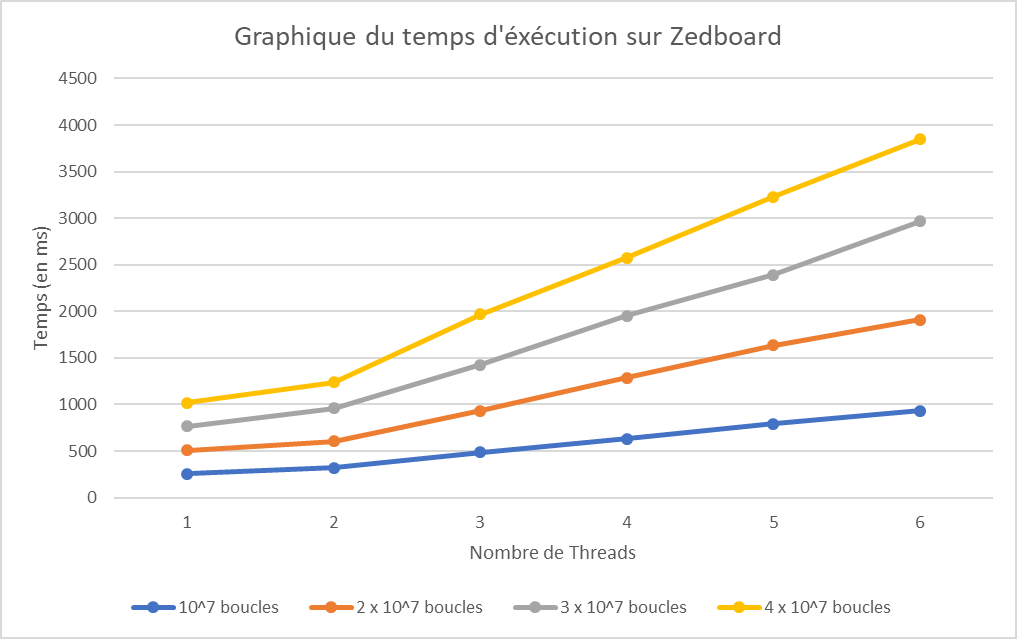
\includegraphics[width=\textwidth]{graph.png}
\end{figure}

\paragraph{Question 2c} Done (\texttt{main\_td2c.cpp}). When not using a mutex, the inaccuracies observed in question 2a are still observed, which is consisted since we're essentially running the same program. When using a mutex, no such inaccuracies are observed and the final value of the counter is exactly $\texttt{nLoops}\cdot\texttt{nTasks}$. The version using a mutex is much slower than the one without (by a factor of roughly 25 for 1,000,000 loops and 50 tasks).

We conclude that a mutex allows us to protect the counter (or other ressources) from concurrent accesses, at the cost of decreased performance.

\textbf{Note.} For this question, \texttt{g++} issues a warning about a missing initialiser for member \texttt{mutex} (of type \texttt{pthread\_mutex\_t}) of structure \texttt{ThreadData}. Since this member must be manually initialised using the POsix function \texttt{pthread\_mutex\_init}, the warning is irrelevant.

\section*{TD3}
\paragraph{Question 3a} The Chrono class can be found in files \texttt{Chrono.h} and \texttt{Chrono.cpp}. A sample main file, which illustrates some functionalities of the class, can be found in \texttt{main\_td3a.cpp}. As far as we can tell by counting seconds on a wrist-watch, it is working fine.

\paragraph{Question 3b} The Timer class can be found in files \texttt{Timer.h} and \texttt{Timer.cpp}; the PeriodicTimer class in files \texttt{PeriodicTimer.h} and \texttt{PeriodicTimer.cpp}.

The constructor, destructor, \texttt{start} and \texttt{stop} methods of the Timer class need be public because the user needs access to these functionalities. The destructor must be virtual since we use inheritance, the \texttt{start} method must also be virtual since derived classes may need to override it.

The \texttt{callback} method of the Timer class must be protected and virtual since we do not want the user to be able to access it and derived classes will need access to override that of the base class (it is not implemented in the base class).

The \texttt{call\_callback} method of the Timer class must be private (since we do not want the user to either be aware of it or use it manually). It must be static since the signature of the handler is determined by the Posix API, and therefore may not be a class method.

The \texttt{tid} attribute of the Timer class must be protected since the user shall not be able to access it and derived classes will need access.

The \texttt{start} method of the PeriodicTimer class is public since it overrides a public method of the base class.

The CountDown class can be found in files \texttt{CountDown.h} and \texttt{CountDown.cpp}, the main file is \texttt{main\_td3b.cpp}.

\paragraph{Question 3c} The Calibrator class can be found in files \texttt{Calibrator.h} and \texttt{Calibrator.cpp}; the CpuLoop class in files \texttt{CpuLoop.h} and \texttt{CpuLoop.cpp}; the Looper class in files \texttt{Looper.h} and \texttt{Looper.cpp}. File \texttt{main\_td3c.cpp} makes the above classes.

\section*{TD4}
\paragraph{Question 4a} The custom thread class (derived from our \texttt{thread} class) can be found in files \texttt{IncrThread.h} and \texttt{IncrThread.cpp}. The main file is \texttt{main\_td4a.cpp}.

\paragraph{Question 4b} The custom thread class (derived from our \texttt{thread} class) can be found in files \texttt{SafeIncrThread.h} and \texttt{SafeIncrThread.cpp}. The main file is \texttt{main\_td4b.cpp}.

\paragraph{Question 4c} The Semaphore class can be found in files \texttt{Semaphore.h} and \texttt{Semaphore.cpp}. A producer-consumer pattern is implemented in \texttt{main\_td4c.cpp}. Our tests have shown that all produced tokens are consumed.

\paragraph{Question 4d} The Fifo template can be found in file \texttt{Fifo.h} (the use of a template is dictated by the necessity to be able to store any one type of data in the structure). A producer-consumer pattern is implemented in \texttt{main\_td4d.cpp}. Our tests have shown that all produced tokens are consumed.

\end{document}
